\documentclass[12pt,a4paper,twoside,openright]{book}
\usepackage{lmodern} % font
\usepackage[english]{babel}
\usepackage{csquotes}
\usepackage{lipsum, kantlipsum}
\usepackage{etoolbox}

% For Title styling
\usepackage{titlesec}
\titleformat*{\section}{\LARGE\bfseries}
\titleformat*{\subsection}{\Large\bfseries}
\titleformat*{\subsubsection}{\large\bfseries}

% Margins and layout
\usepackage[margin=2.5cm]{geometry}
\usepackage{setspace}
\onehalfspacing % Increase the line spacing
\setlength{\headheight}{14.5pt}

% Graphics and figures
\usepackage{graphicx}
\usepackage{float}
\graphicspath{{figures/}}

% Mathematics
\usepackage{amsmath,amssymb,amsthm}
% Physics
\usepackage{braket}

% Bibliography
\usepackage[backend=biber,style=numeric,sorting=none]{biblatex}
\addbibresource{bibliography.bib}

% Hyperlinks
\usepackage[colorlinks=true,linkcolor=black,citecolor=blue,urlcolor=blue]{hyperref}

% Headers and footers
\usepackage{fancyhdr}
\usepackage{extramarks}
\pagestyle{fancy}
\fancyhf{}
\fancyhead[LE,RO]{\thepage} % Left Even, Right Odd number page
\fancyhead[RE]{\leftmark}   % Right Even, left mark (Chapter title)
\fancyhead[LO]{\rightmark}  % Left Odd, right mark (Section name)


% No indentation on new paragraphs
\setlength{\parindent}{0pt}

% For organizing the work in subfiles
\usepackage{subfiles}

% For numbering also subsubsections
\setcounter{secnumdepth}{3}
\setcounter{tocdepth}{3}

% Tikz 
\usepackage{tikz}
\usetikzlibrary{calc, positioning, arrows.meta}
\usepackage{xcolor}
\usepackage{optikz}

\begin{document}

%* #########################################################
%* ### Title page
\input{Title page/titlepage}
\thispagestyle{empty}

%* #########################################################
%* ### Citation Page
% Front matter (use roman number for page)
\frontmatter 
\thispagestyle{empty}
    \vspace*{6cm}
    \begin{flushright}
        \textit{Pokémon forti, Pokémon deboli.\\ Sono distinzioni dettate dall’egoismo. \\ Gli allenatori davvero in gamba dovrebbero vincere coi loro preferiti.}

        \vspace{\baselineskip}
        \textit{Strong Pokémon, weak Pokémon.\\ That is only the selfish perception of people.\\ Truly skilled trainers should try to win with their favorites.}

        \vspace{\baselineskip}
        \textit{Karen, Johto Elite Four}
    \end{flushright}
    
    \newpage
    \thispagestyle{empty}

	\tableofcontents
    \newpage
    \thispagestyle{empty}

% Main content (Use Arabic number for pages)
\mainmatter

%* #########################################################
%* ### Introduction
\subfile{chapters/Introduction/introduction.tex}

%* #########################################################
%* ### Chapter 1
\subfile{chapters/Chapter_1/chapter_1_main.tex}

%* #########################################################
%* ### Chapter 2
\subfile{chapters/Chapter_2/chapter_2_main.tex}

%* #########################################################
%* ### Chapter 3
\subfile{chapters/Chapter_3/chapter_3_main.tex}

%* #########################################################
%* ### Appendix
% \appendix

% \begin{figure}
%     \centering
%     \begin{subfigure}{0.49\linewidth}
%         \centering
%         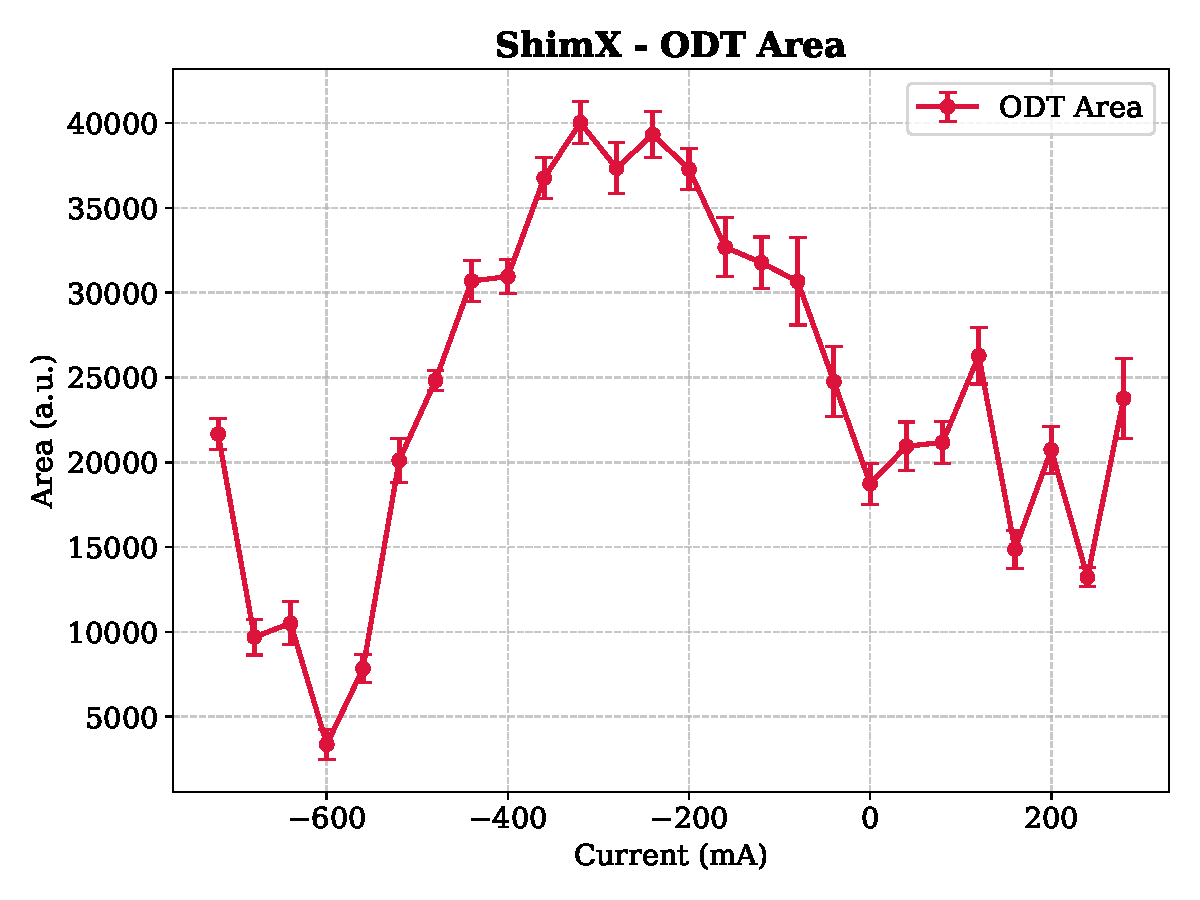
\includegraphics[width=\linewidth]{Cap_3_figures/ODT_loading/final_results/ShimX/shimX_signal_g_area.pdf}
%         \caption{}
%         \label{fig:shimX_signal}
%     \end{subfigure}
%     \begin{subfigure}{0.49\linewidth}
%         \centering
%         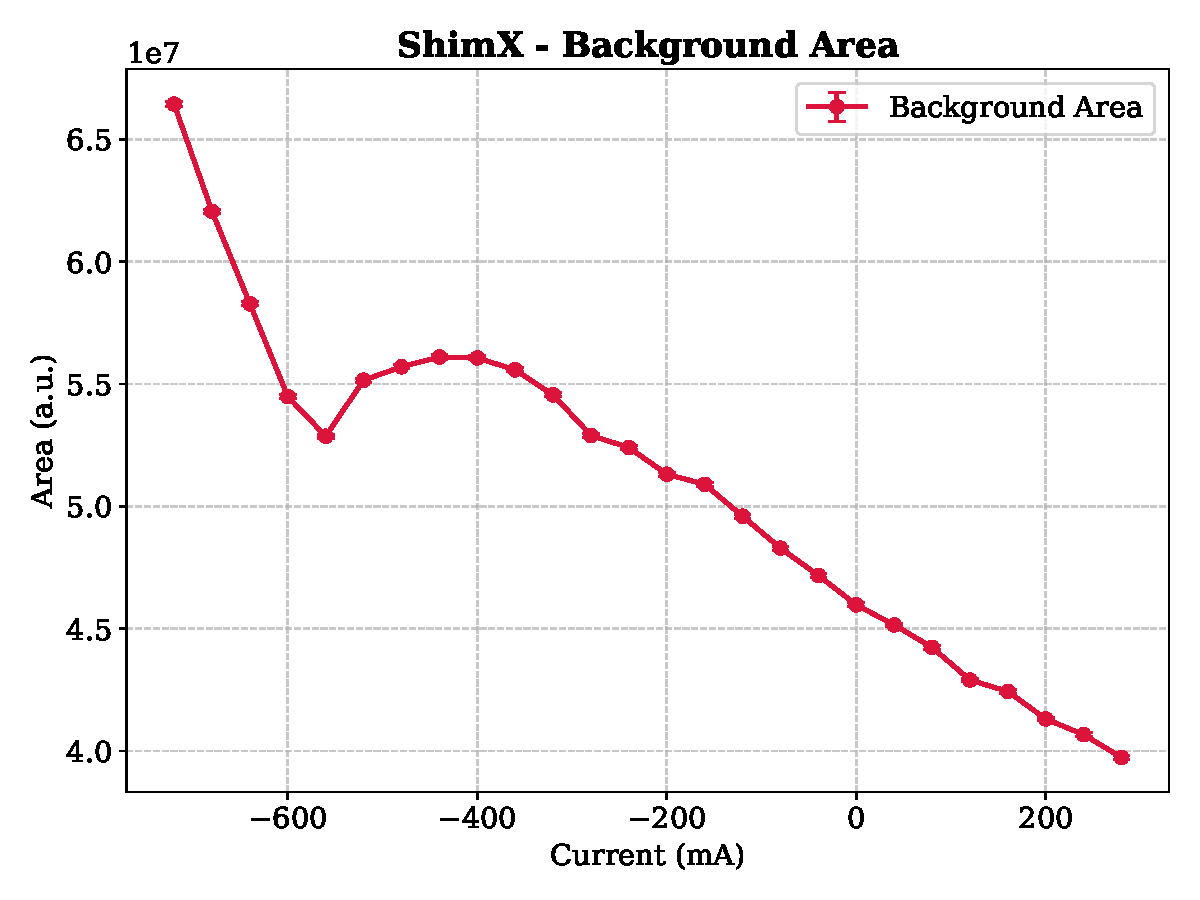
\includegraphics[width=\linewidth]{Cap_3_figures/ODT_loading/final_results/ShimX/shimX_bkg_g_area.pdf}
%         \caption{}
%         \label{fig:shimX_bkg}
%     \end{subfigure}
    
%     \begin{subfigure}{0.49\linewidth}
%         \centering
%         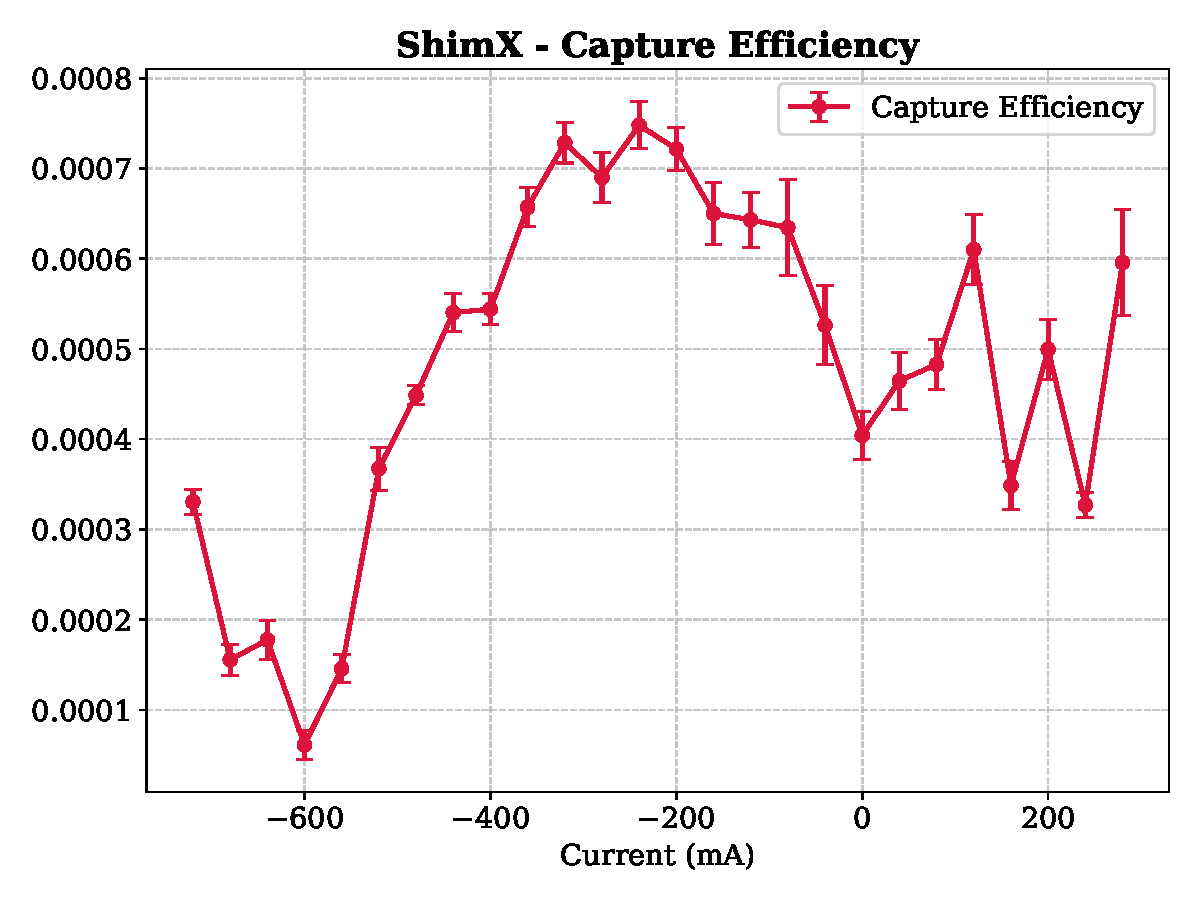
\includegraphics[width=\linewidth]{Cap_3_figures/ODT_loading/final_results/ShimX/shimX_capture_efficiency.pdf}
%         \caption{}
%         \label{fig:shimX_efficiency}
%     \end{subfigure}
%     \caption{Optimization results for the x-compensation coil current: (a) ODT signal area, (b) background area, (c) capture efficiency.}
%     \label{fig:shimX_results}
% \end{figure}

% \begin{figure}
%     \centering
%     \begin{subfigure}{0.49\linewidth}
%         \centering
%         
\includegraphics[width=\linewidth]{Cap_3_figures/ODT_loading/final_results/ShimZ/shimZ_signal_g_area.pdf}
%         \caption{}
%         \label{fig:shimZ_signal}
%     \end{subfigure}
%     \begin{subfigure}{0.49\linewidth}
%         \centering
%         
\includegraphics[width=\linewidth]{Cap_3_figures/ODT_loading/final_results/ShimZ/shimZ_bkg_g_area.pdf}
%         \caption{}
%         \label{fig:shimZ_bkg}
%     \end{subfigure}

%     \begin{subfigure}{0.49\linewidth}
%         \centering
%         
\includegraphics[width=\linewidth]{Cap_3_figures/ODT_loading/final_results/ShimZ/shimZ_capture_efficiency.pdf}
%         \caption{}
%         \label{fig:shimZ_efficiency}
%     \end{subfigure}
%     \caption{Optimization results for the z-compensation coil current: (a) ODT signal area, (b) background area, (c) capture efficiency.}
%     \label{fig:shimZ_results}
% \end{figure}

% \begin{figure}
%     \centering
%     \begin{subfigure}{0.49\linewidth}
%         \centering
%         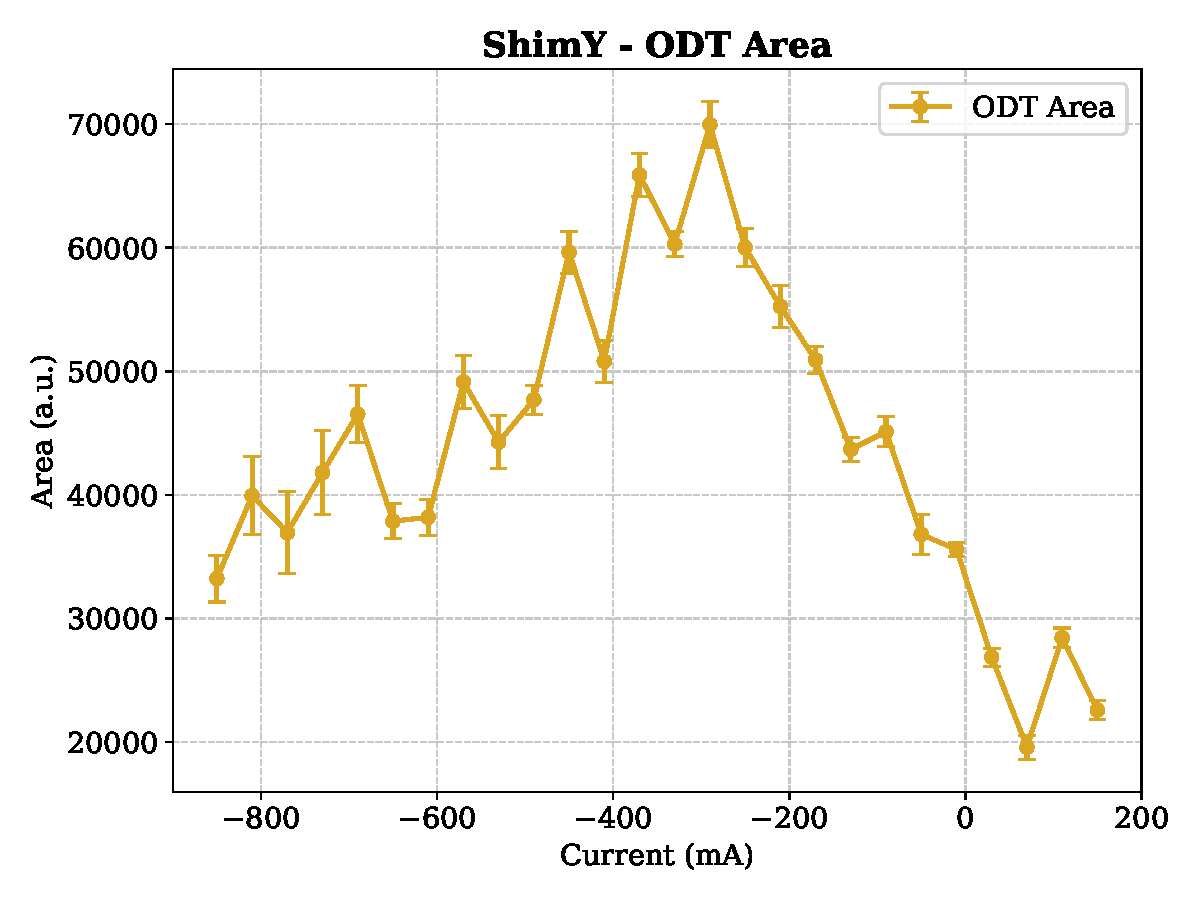
\includegraphics[width=\linewidth]{Cap_3_figures/ODT_loading/final_results/ShimY/shimY_signal_g_area.pdf}
%         \caption{}
%         \label{fig:shimY_signal}
%     \end{subfigure}
%     \begin{subfigure}{0.49\linewidth}
%         \centering
%         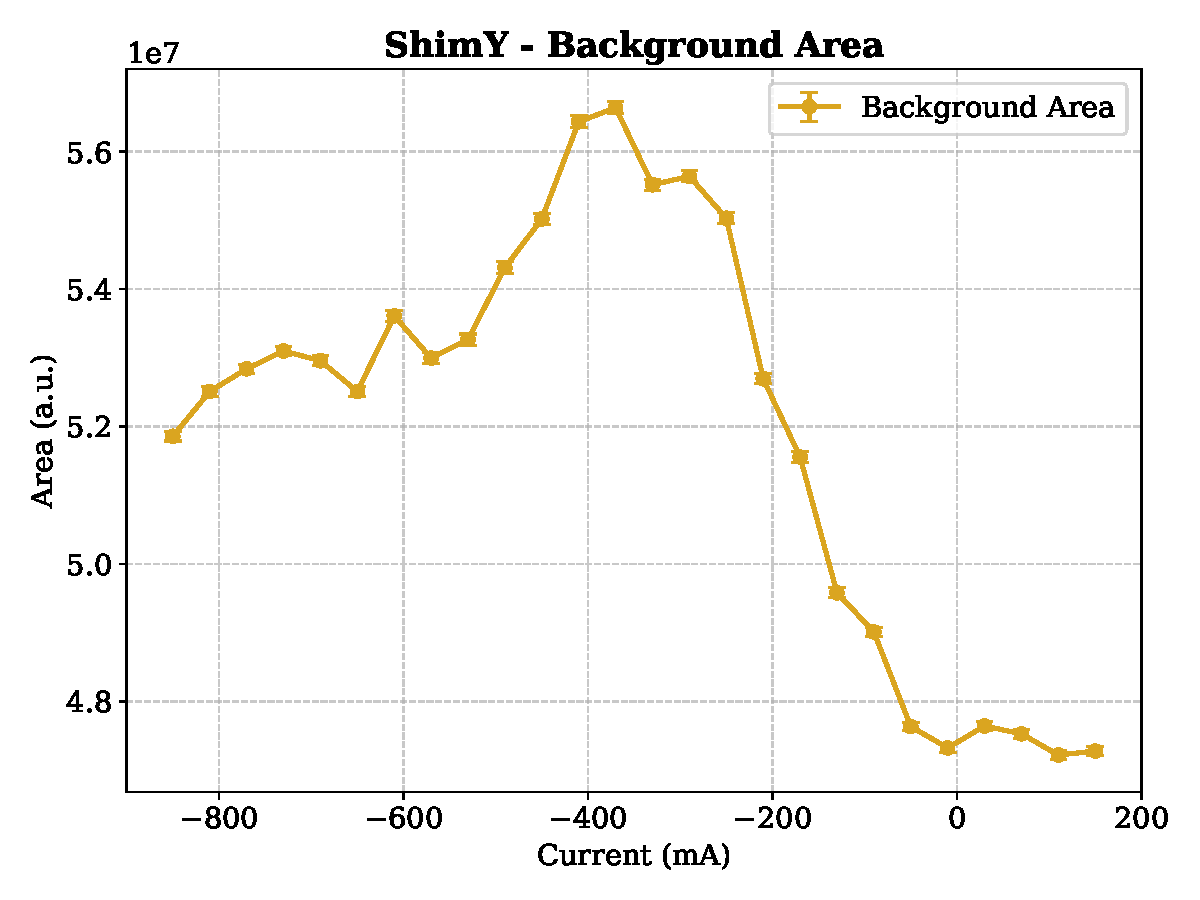
\includegraphics[width=\linewidth]{Cap_3_figures/ODT_loading/final_results/ShimY/shimY_bkg_g_area.pdf}
%         \caption{}
%         \label{fig:shimY_bkg}
%     \end{subfigure}

%     \begin{subfigure}{0.49\linewidth}
%         \centering
%         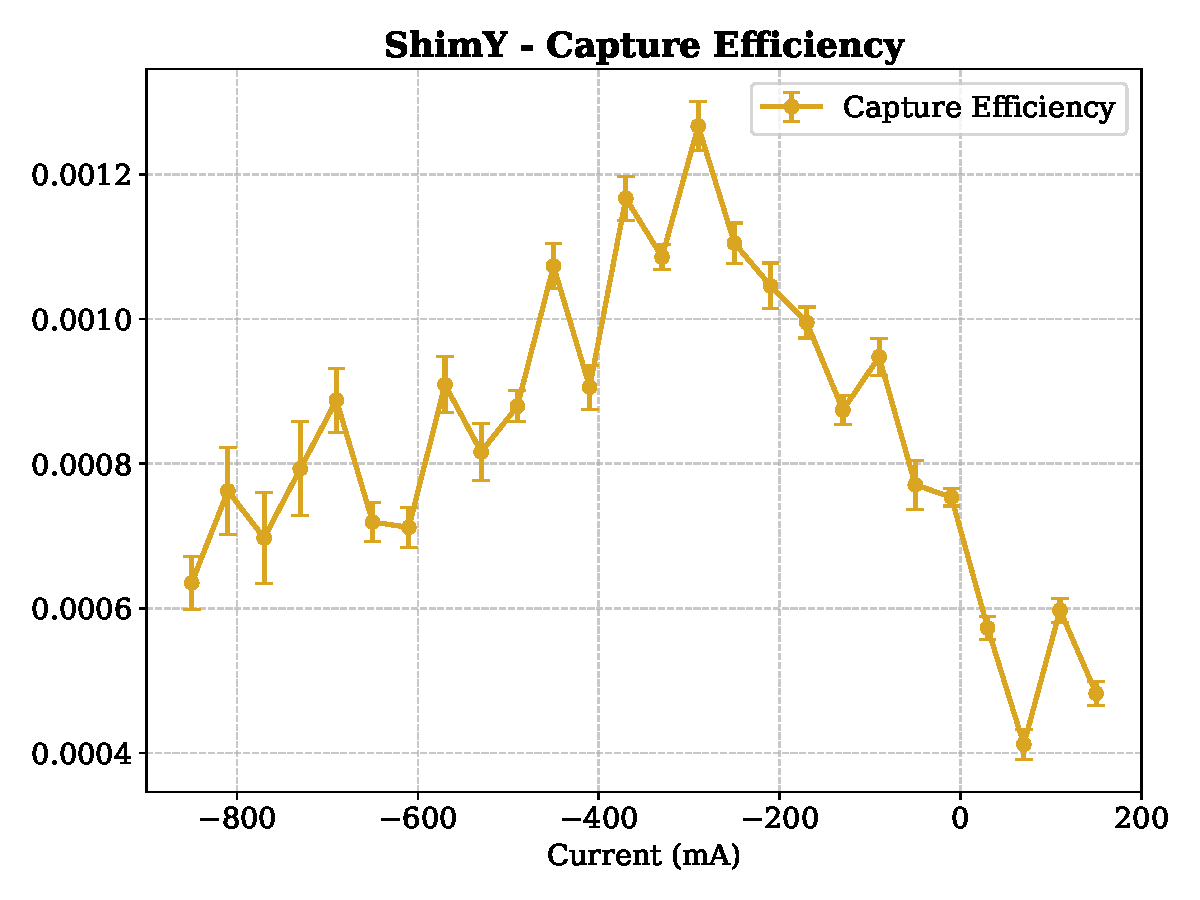
\includegraphics[width=\linewidth]{Cap_3_figures/ODT_loading/final_results/ShimY/shimY_capture_efficiency.pdf}
%         \caption{}
%         \label{fig:shimY_efficiency}
%     \end{subfigure}
%     \caption{Optimization results for the y-compensation coil current: (a) ODT signal area, (b) background area, (c) capture efficiency.}
%     \label{fig:shimY_results}
% \end{figure}

\printbibliography
\end{document}
